\section{Документация к программе}

Документация к программе является важнейшей составляющей процесса разработки программного обеспечения. В рамках нашей курсовой работы мы уделили значительное внимание созданию подробной и качественной документации для API нашего приложения, используя OpenAPI.

\textbf{OpenAPI} — это язык описания RESTful API, который позволяет разработчикам определять все доступные ресурсы, методы, параметры и схемы данных, используемые в приложении. Благодаря OpenAPI, разработка и поддержка API становится более структурированной и стандартизированной, что упрощает процесс интеграции с другими системами.

Для визуализации и тестирования API мы использовали \textbf{Swagger UI}. Этот инструмент предоставляет удобный интерфейс для просмотра документации, а также позволяет разработчикам выполнять тестовые запросы к API непосредственно из браузера. На рисунке \ref{swagger} представлен пример отображения документации нашего API в Swagger UI. Здесь показаны все доступные ресурсы, методы и параметры, а также имеется возможность протестировать каждый метод в реальном времени.

Использование OpenAPI и Swagger UI принесло множество преимуществ:
\begin{itemize}
    \item \textbf{Стандартизация:} OpenAPI обеспечивает единый стандарт для описания API, что облегчает понимание и использование API как внутри команды, так и для внешних разработчиков.
    \item \textbf{Удобство поддержки:} Благодаря четкой структуре и автоматической генерации документации, процесс поддержки и обновления API значительно упрощается.
    \item \textbf{Интеграция:} Наличие подробной документации облегчает интеграцию нашего API с другими приложениями и системами.
\end{itemize}

Таким образом, внедрение OpenAPI для документирования нашего API позволило не только повысить качество и удобство работы с API, но и упростить процесс интеграции, обеспечивая высокий уровень стандартизации и прозрачности.

\begin{figure}[h]
    \centering
    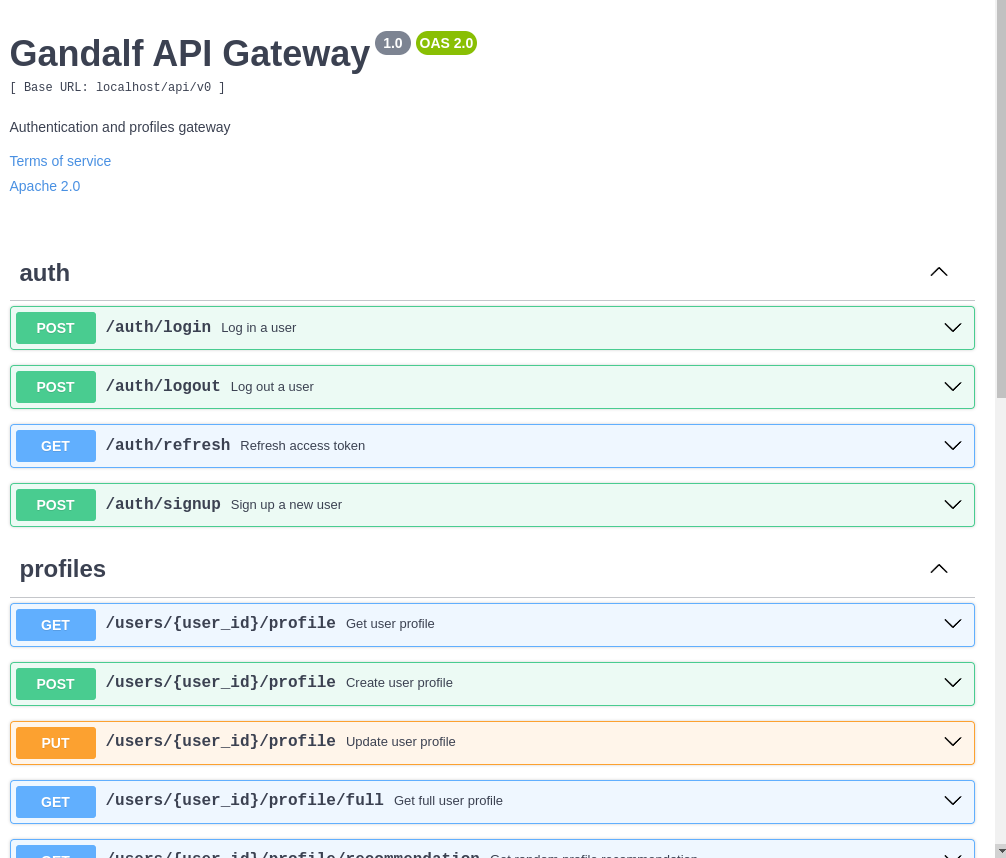
\includegraphics[width=1\linewidth]{swagger_editor_screen.png}
    \caption{Пример документации API в Swagger UI}
    \label{swagger}
\end{figure}